%%% gssa.tex --- 


\section{Background}

The analysis of adaptation at large or complete genome scale is currently based on concepts and methods developed for single genes analyzes~\cite{Arbiza2006,Bakewell2007,Bustamante2005,Clark2003,Nielsen2005}. Statistical methods to test for neutrality~\cite{Nielsen2001}, are currently used without considering if genes works independently or associated to others to produce a single phenotypic response. In this sense we are applying pre-genomics concepts and methods to genomics data. The current paradigm for large scale analysis of adaptation consists in a two steps framework: first, the search for a list of genes (in a gene-by-gene framework analysis) with a statistical significant signal of positive selection ($\omega > 1$), and second, the search for over-represented functional classes of genes in this list. Although it is logically consistent, it has been noted that this kind of strategy causes an enormous loss of information due to the large number of false negatives that are accepted in order to preserve a low ratio of false positives necessary when genomics data is considered~\cite{Al-Shahrour2007,Al-Shahrour2005a,Al-Shahrour2006,Subramanian2005}.

Genes do not operate alone within the cell, but in a intricate network of interactions that we have only recently started to envisage~\cite{Stelzl2005}. It is a widely accepted fact that coexpressing genes tend to be fulfilling common roles in the cell~\cite{Lee2003}. Moreover, coexpression seems to occur, in many cases, in contiguous chromosomal regions~\cite{Caron2001} and furthermore, recent evidences suggest that functionally related genes map close in the genome, even in higher eukaryotes~\cite{Hurst2004}. Many higher-order levels of interaction are continuously being discovered and even complex traits, including diseases, have started to be considered from a systems biology perspective~\cite{Ideker2008,Vamathevan2008}.

Recent methodology was proposed to circumvent the classical two-step analysis as a new attempt to test for selective signatures across species at genome-scale level~\cite{Shapiro2008} Using the deviations of the expected rates of evolution for a large group of genes in a group of gamma proteobacteria, the authors conclude that the coherence of selective patterns suggests that the genomic landscape is organized into functional modules even at the level of natural selection.

The hypothesis we aim to test in this study is not about individual genes, but about functional classes. Mutations occur on single genes but natural selection acts on phenotypes by operating on whole sub-cellular systems. Mutations in genes either remain finally fixed or disappear because of their beneficial or disadvantageous effect on individual fitness, respectively. This effect on the function of individual proteins can only be understood in the context of the system (e.g. a pathway, GO functional roles, etc.) in which the proteins are involved. If a list of genes arranged by some parameter that accounts for their evolutionary rates is examined, it is expected that genes belonging to pathways or functional classes favored or disfavored by selection will tend to appear towards the extremes.

This approach circumvents the implicit assumption posed by the two-step analysis described above assuming by that the gene is the only target of selection. If natural selection works by means of minor quantitative effects of many different changes distributed along different gene products most of them working together in a few number of systems (GO functional terms, biochemical pathways and/or interactome modules) we expect to find: \begin{inparaenum}[ 1-] \item correlated nonsynonymous rate changes associated to these functions , \item synonymous rate changes not necessarily associated to the same functions, \item a higher number of significant functions than those discovered in the classical two-step approach.\end{inparaenum}

In the first part of this paper we extend the classical two-step approach previously reported by us for human and chimp \cite{Arbiza2006}, to rat and mouse now considering a set of XXXX orthologous genes of human, chimpanzee, mouse, rat and dog. The objective is to compare the classical two-step approach with the new system approach developed in the second part of the paper. In both cases we search for differences in evolutionary rates differentiating positive selection from relaxation along the branches of the phylogeny of the species.

\section{Material and Methods}

\subsection{Orthology prediction}

Complete genomes of 5 mammals species (\textit{Homo sapiens}, \textit{Pan troglodytes}, \textit{Mus musculus}, \textit{Rattus norvegicus} and \textit{Canis familiaris}) where retrieved from \textit{Ensembl} \cite{Flicek2011}. Also orthology prediction between each pair of species possibly done between human and the others was retrieved from \textit{Ensembl Compara} \cite{Vilella2009} using biomart \cite{Kinsella2011} and taking human as \gls{seed} species. Only groups of orthologs \textit{one-to-one} with one representative of each species where kept in the final dataset \fref{fig:phylogeny}{-A}.

\begin{figure}[htpb] 
\centering 
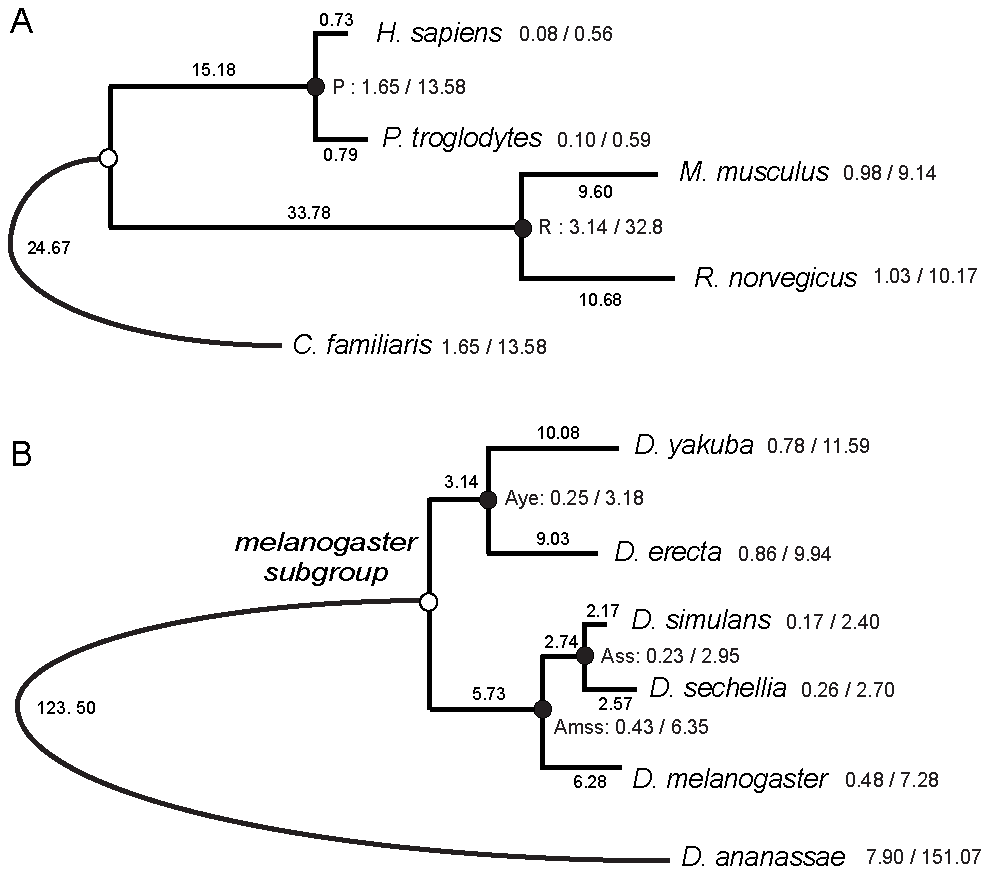
\includegraphics[width=\textwidth]{tex_source/figures/gssa/phylogenies.png}
\caption[Mammals and \textit{Drosophila} phylogeny]{{\bf Mammals and
 \textit{melanogaster} group phylogeny.} \\Numbers on internal and external nodes represent the median number of nonsynonymous and synonymous substitutions per codon (dN/dS) estimated from all the coding sequences compared in mammal (A) and Drosophila (B) genomes. Branch lengths and rates were multiplied by 100. Ancestral estimation of parameters was done in primates (P), rodents (R), D. yakuba and D. erecta (Aye), D. simulans and D. sechellia (Ass), and D. melanogaster, D. simulans and D. sechellia (Amss). C. familiaris and D. ananassae were chosen as outgroup species in the corresponding tree.} 
\label{fig:phylogeny}
\end{figure}

The same procedure was applied for \textit{melanogaster} group, including 6 species namely, \textit{Drosophila melanogaster} (as \gls{seed}-species), \textit{Drosophila sechelia}, \textit{Drosophila simulans}, \textit{Drosophila yakuba}, \textit{Drosophila erecta} and, as outgroup, \textit{Drosophila ananassae} (see \fref{fig:phylogeny}{-B}).

\subsection{Alignments refinement and filters}
DNA coding sequences (CDS) were aligned according to protein translation pattern using \textit{Muscle} version 3.7 \cite{Edgar2004} embedded into the \textit{CDS-Protal} utility in \textit{Phylemon 2.0} \cite{Sanchez2011}, and to avoid the presence of badly aligned regions alignments were cleaned using \textit{TrimAl} \cite{Capella-Gutierrez2009} keeping all sequences but trimming alignment columns with the heuristic method \textit{automated-1}. Additionally, alignments smaller than 100 bp were excluded from the analysis. 

In mammals, the upper limit for dN and dS considered was those of the human interferon $\gamma$ (dN = 3.06) and the relaxin protein \cite{Graur2000} (dS = 6.39 substitutions per site per 1e9 years). Assuming the human-mouse, mouse-rat and human-chimp differentiation times to be about 80, 70 and 5 million years \cite{BlairHedges2003}, respectively, ortholog comparisons between primates and rodents with dS$\ge$1 and dN$\ge$0.5, rodents with dS$\ge$0.256, dN$\ge$0.122, and primates with dS$\ge$0.064 and dN$\ge$0.030 substitutions/site were excluded.

The number of orthologs kept for analysis after filtering steps, is 12,453 for mammals, and 9,240 for flies.

\subsection{Evolutionary analysis}

Maximum likelihood estimation of dN, dS, and $\omega$ was computed using CodeML program from PAML \cite{Yang2007}. Evolutionary rates were computed in orthologous sequences according to the free-ratio branch model assuming independent $\omega$ ratio for each branch of the tree of mammals and Drosophila species (see raw values of rates in Table S1 and S2). Evolutionary rates (dN, dS), its ratio ($\omega$), and its difference between ancestral and descendant species ($\delta\omega$) were ranked along all genes of genomes and further analyzed by GSSA.

External branches of Figure 1 were labeled as foreground to test for positive selection using branch-site models in Test I and Test II \cite{Zhang2005}. Positive results of relaxation of selective constraints (or weak signals of positive selection) were discarded \cite{Arbiza2006}. To quantify the relative contribution of PSGs in functional modules showing SH$\omega$ and SL$\omega$ results in GSSA, a t-test (from R package \cite{Ihaka1996}) with the mean number of PSGs per functional modules was computed in primates, rodents, mammals and Drosophila species. An independent set of PSGs was collected to test the robustness of our results in mammals \cite{Kosiol2008a}, and Drosophila species \cite{Clark2007}.

\subsection{GSSA, evolutionary and statistical simulations}

Gene-set selection analysis across lists of genes ranked by different evolutionary rate parameters (dS, dN, $\omega$ and $\delta\omega$) was computed using the program Babelomics \cite{Al-Shahrour2008}. This program implements a version of GSA \cite{Al-Shahrour2005a} which can be applied to any list of ranked genes regardless of the initial experimental design \cite{Dopazo,Huang2009}. The aim of the test is to find functional classes, namely blocks of genes that share some functional property, showing a significant asymmetric distribution towards the extremes of a list of ranked genes. This is achieved by means of a segmentation test, which consists on the sequential application of a Fisher's exact test over the contingency tables formed with the two sides of different partitions (A and B in Figure 2) made on an ordered list of genes. The two-tailed Fisher's exact test finds significantly over or under represented functional classes when comparing the upper side to the lower side of the list, as defined by any partition (in Figure 2, four of the five partitions show significant differences). Similarly to other equivalent gene-set analyses, the outcomes are those modules (GO and KEGG) significantly associated to high or low values of the evolutionary parameter used to rank the genes. Previous results showed that a number between 20 and 50 partitions often gives optimal results in terms of sensitivity and results recovered [18]. Here we applied 30 partitions along all the GSSA performed. Given that multiple functional classes (C) are tested in multiple partitions (P), the unadjusted p-values for a total of C $\cdot$ P tests were corrected by the widely accepted FDR method \cite{Benjamini2001}.

Originally, 1,394/1,331 GO terms, and 199/116 KEGG pathways were analyzed in mammals and Drosophila species respectively. The global GO directed acyclic graph was processed with Blast2GO \cite{Conesa2005} to extend the annotation at missing parental nodes, discarding GO levels out of 2 to 8 for mammals, and 2 to 12 for Drosophilas. The final set of GO and KEGG terms used in the GSSA corresponds to those containing a minimum number of 15 genes. To test possible biases attributed to the size of the functional category, the magnitude of change in evolutionary rate or the proportion of genes experiencing a rate change we randomized the original assignation of ENSG's to the list of ranked values and functional annotation (see Figure S5A). For each evolutionary variable and species 10.000 randomizations and the corresponding GSSA were performed. The proportion of false positives (significant results after GSSA) was computed for each evolutionary variable and plotted along the size of functional categories (from 20 to 1,400 with intervals of 20). Because this proportion never reached values higher than 0.5\% (FDR) we rejected the possibility that either group size or rate distribution biased GSSA results in our data set (see Figure S5A and S5B-C).

Finally, in order to validate the independence of the GSSA from the effects of alternative evolutionary constraints we simulated selective regimes (purifying selection, positive selection and relaxation of selective constraints) using branch-site models. Here we addressed the possibility of a variation in the representation of significant results after GSSA (see Supplementary Figure S6). We found that when a massive enrichment of genes under each of the evolutionary scenarios described take place in the genome, none of them bias the results of GSSA (see Text S1).

\section{open on colocalization to not random}

%%% Local Variables: 
%%% mode: latex
%%% TeX-master: "../../master"
%%% End: 
